\section{\uppercase{Optimization of the combination step of EAC}}
\label{sec:combination}

Space complexity is the main challenge building the co-association matrix.
A complete pair-wise co-association matrix has $O(n^2)$ complexity but can be reduced to $O(\frac{n(n-1)}{2})$ without loss of information, due to its symmetry.
Still, these complexities are rather high when large datasets are contemplated, since it becomes infeasible to fit these co-association matrices in the main memory of a typical workstation.
% Two solutions in literature address this challenge.
%\cite{Fred2005} approaches it by using a $k$-Nearest Neighbor approach, only considering associations between the $k$ closest neighbors of each pattern.
\cite{Lourenco2010} approaches the problem by exploiting the sparse nature of the co-association matrix, but doesn't cover the efficiency of building a sparse matrix or the overhead associated with sparse data structures.
The effort of the present work was focused on further exploiting the sparse nature of EAC, building on previous insights and exploring the topics that literature has neglected so far.

Building a non-sparse matrix is easy and fast since the memory for the whole matrix is allocated and indexing the matrix is direct.
When using sparse matrices, neither is true.
In the specific case of EAC, there is no way to know what is the number of associations the co-association matrix will have which means it is not possible to pre-allocate the memory to the correct size of the matrix.
This translates in allocating the memory gradually which may result in fragmentation, depending on the implementation, and more complex data structures, which incurs significant computational overhead.
For building a matrix, the DOK (Dictionary of Keys) and LIL (List of Lists) formats are recommended in the documentation of the SciPy \cite{JonesSciPy} scientific computation library.
%The DOK (Dictionary of Keys) and LIL (List of Lists) sparse formats 
These were briefly tested on simple EAC problems and not only was their execution time several orders of magnitude higher than a traditional fully allocated matrix, but the overhead of the sparse data structures resulted in a space complexity higher than what would be needed to process large datasets.
For operating over a matrix, the documentation recommends converting from one of the previous formats to either CSR (Compressed Sparse Row) or CSC (Compressed Sparse Column).
%The CSR (Compressed Sparse Row) is another sparse format, but is more adequate for computations, not matrix building.
Building with the CSR format had a low space complexity but the execution time was much higher than either one of the other sparse formats.

The bad performance of the above sparse formats combined with the fact that no relevant literature was found on efficiently building sparse matrices, led to the design and implementation of a novel strategy for a CSR matrix specialized to the EAC context, the \textbf{EAC CSR}.

\subsection{Underlying structure of EAC CSR}

The first step of EAC CSR is making an initial assumption on the maximum number of associations \emph{max\_assocs} that each pattern can have.
A possible rule is $$max\_assocs = 3 \times bgs$$ where $bgs$ is the biggest cluster size in the ensemble.
The biggest cluster size is a good heuristic for trying to predict the number of associations, since it is the limit of how many associations each pattern will have in any partition of the clustering ensemble.
Furthermore, one would expect that the neighbors of each pattern will not vary significantly, i.e. the same neighbors will be clustered together repeatedly in many partitions.
This scheme for building the matrix uses 4 supporting arrays ($n$ is the number of patterns):

\begin{itemize}
	\item \textbf{indices} - an array of size $n \times max\_assocs$ that stores the columns of each non-zero value of the matrix, i.e. the destination pattern to which each pattern associates with;
	\item \textbf{data} - an array of size $n \times max\_assocs$ that stores all the non-zero association values;
	\item \textbf{indptr} - an array of size $n$  where the \emph{i-th} element is the pointer to the first non-zero value in the \emph{i-th} row.
	\item \textbf{degree} - an array of size $n$  that stores the number of non-zero values of each row.
\end{itemize}

Each pattern (row) has a maximum of \emph{max\_assocs} pre-allocated that it can use to fill with new associations.
New associations that exceed this pre-allocated maximum are discarded.
%Since each pattern has a maximum pre-defined number of associations, \emph{indptr} does not really need to exist since it can be easily deduced (e.g. $indices[n] = n \times max\_assocs$).
The \emph{degree} array keeps track of the number of associations of each pattern.
Throughout this section, the interval of the \emph{indices} array corresponding to a specific pattern is referred to as that pattern's \emph{indices} interval.
If it is said that an association is added to the end of the \emph{indices} interval, this refers to the beginning of the part of the interval that is free for new associations.
The term indices is used either in the context of the array, in which case it will appear as \emph{indices}, or as the plural of index, in which case it will appear as indices.
Furthermore, it should be noted that this method assumes that the clusters received come sorted in a increasing order.

\subsection{Updating the matrix with partitions}

The first partition is inserted in a special way.
Since it is the first and the clusters are sorted, it is a matter of copying the cluster to the \emph{indices} interval of each of its member patterns, excluding self-associations.
The \emph{data} array is set to 1 on the positions where the associations were added.
Because it is the fastest partition to be inserted, when the whole ensemble is provided at once, the first partition is picked to be the one with the least amount of clusters (more patterns per cluster) so that each pattern gets the most amount of associations in the beginning (on average).
This increases the probability that any new cluster will have more patterns that correspond to already established associations.

For the remaining partitions, the process is different.
For each pattern in a cluster it is necessary to add or increment the association to every other pattern in the cluster.
However, before adding or incrementing any new association, it is necessary to check if it already exists.
This is done using a binary search in the \emph{indices} interval.
This is necessary because it is not possible to index directly a specific position of a row in the CSR format.
Since a binary search is performed $(ns - 1)^2$ times for each cluster, where $ns$ is the number of patterns in any given cluster, the indices of each pattern must be in a sorted state at the beginning of each partition insertion.

\subsection{Keeping the \emph{indices} sorted}

% Two strategies for sorting were devised.
% The \underline{first strategy} is to just insert the new associations at the end of the \emph{indices} array (in the correct interval for each pattern) and then, at the end of processing each partition, use a sorting algorithm to sort all the patterns' intervals in the \emph{indices} array.
% This was easily implemented with existing code, namely using \emph{NumPy}'s \emph{quicksort} implementation, which has an average time complexity of $O(n \log n)$


The implemented strategy results from the observation that, if one could know in which position each new association should be inserted, it would be possible to move all old associations to their final sorted positions and insert the new ones in an efficient manner with minimum number of comparisons (and thus branches in the execution of the code).
For this end, the implemented binary search returns the index of the searched value (key) if it is found or the index for a sorted insertion of the key in the array, if it is not found.
% This means that the position where each new association should be inserted is now available.
New associations are stored in two auxiliary arrays of size $max\_assocs$: one (\emph{new\_assoc\_ids}) for storing the patterns of the associations and the other (\emph{new\_assoc\_idx}) to store the indices where the new associations should be inserted (the result of the binary search).
The process is illustrated with an example in Fig. \ref{fig:normal part}. %, detailed in Algorithm \ref{alg:eac csr sort cluster} and explained in the following paragraph.

\begin{figure}[hbtp]
\centering
% 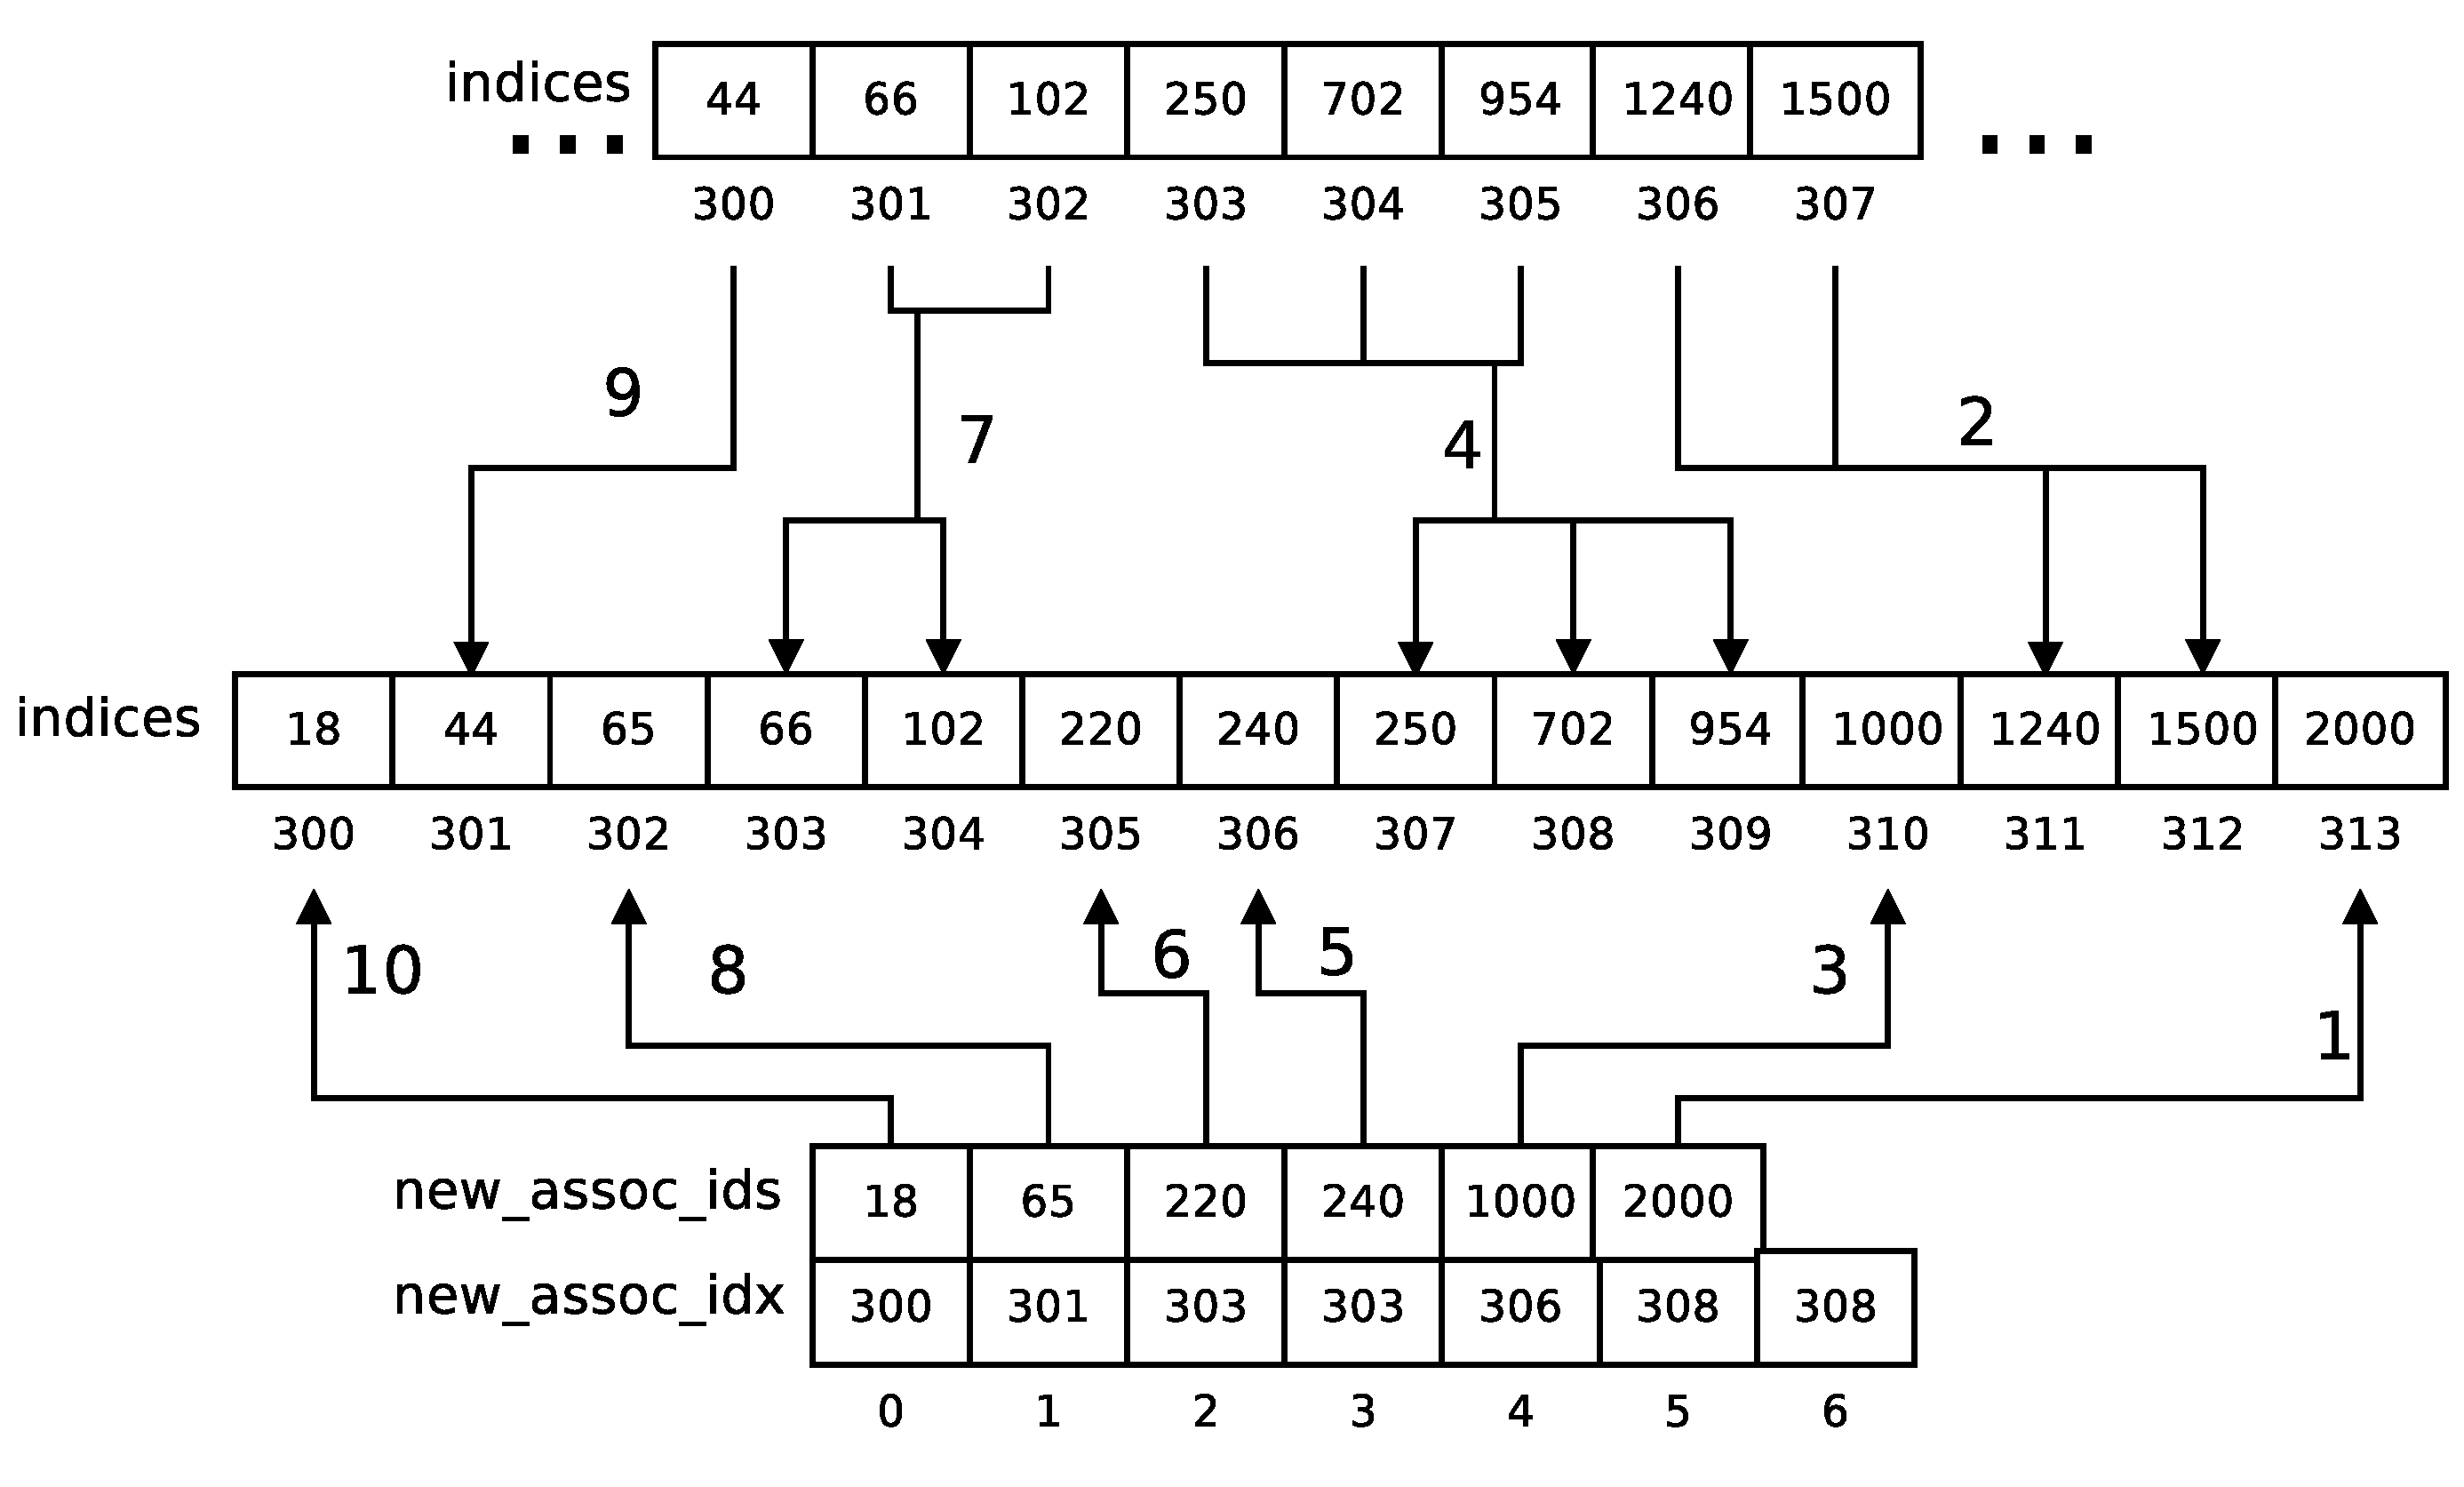
\includegraphics[width=0.45\textwidth]{sorted_insert}
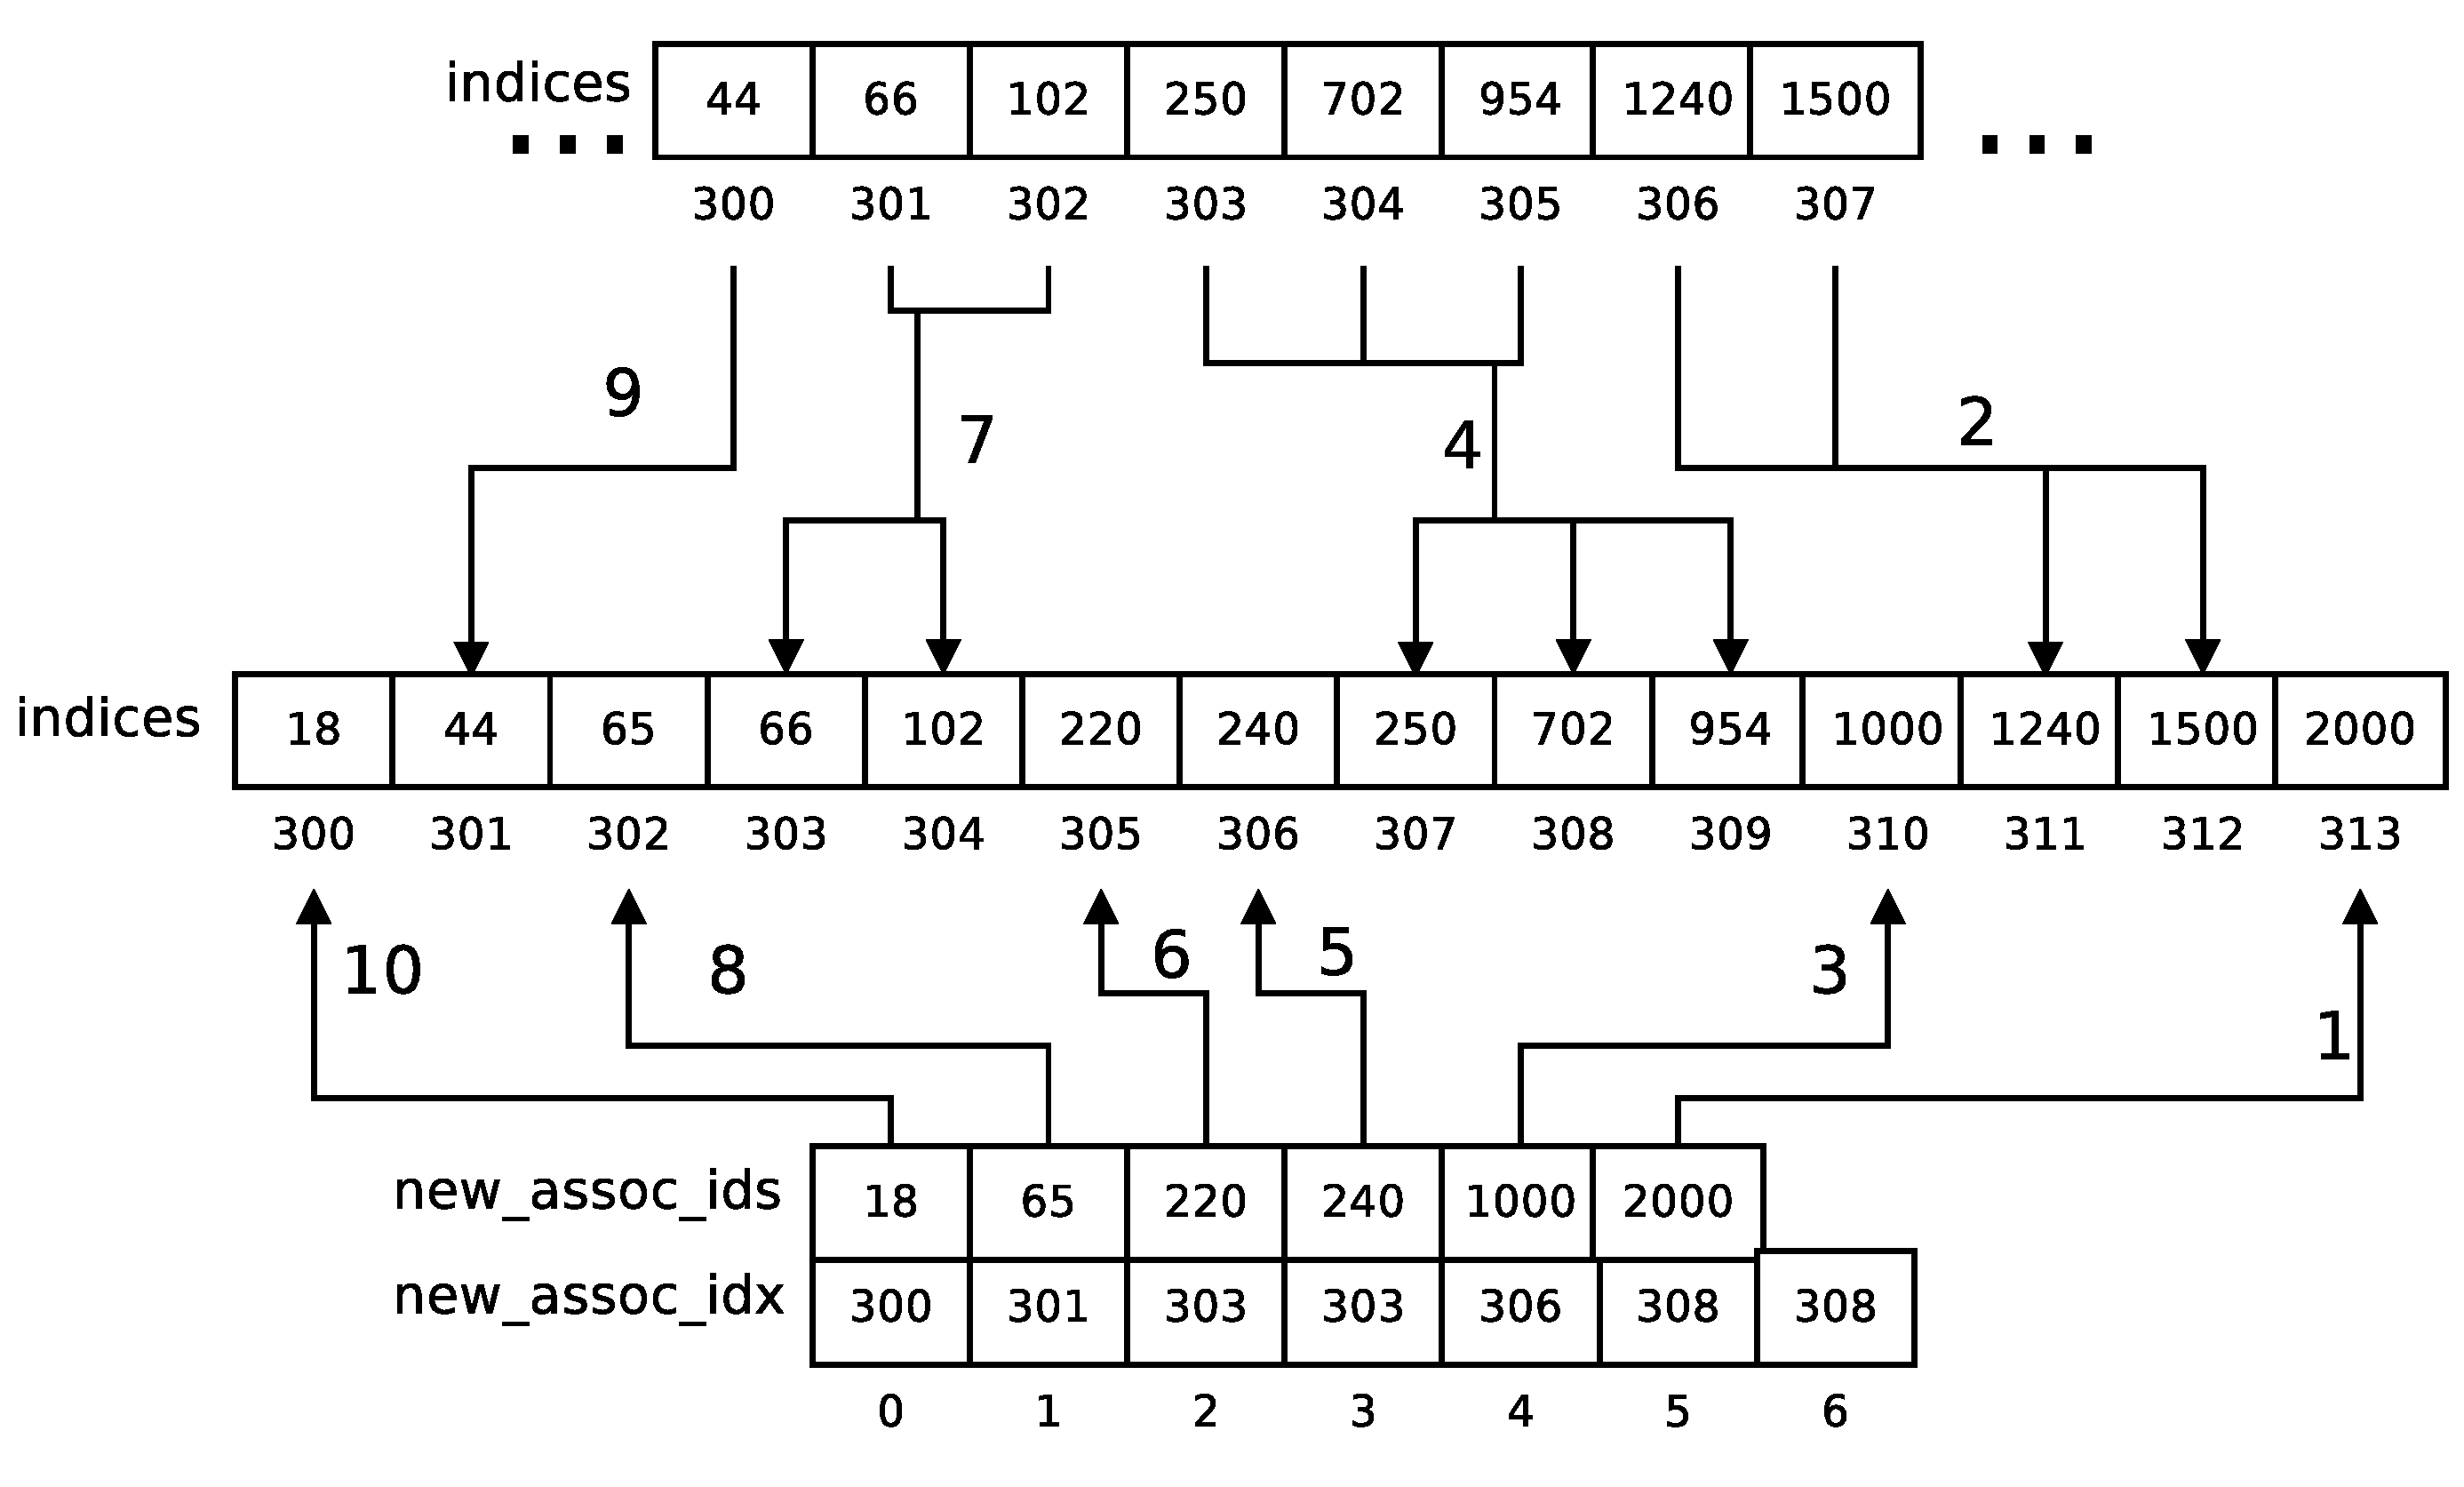
\includegraphics[width=\columnwidth]{sorted_insert}
\caption{Inserting a cluster from a partition in the co-association matrix. The arrows indicate to where the indices are moved. The numbers indicate the order of the operation.}
\label{fig:normal part}
\end{figure}


The binary search operation requires that each pattern's \emph{indices} interval be sorted.
Accordingly, new associations corresponding to each pattern are added in a sorted manner.
%New associations must be added to the pattern's  interval in a sorted manner.
%When updating a partition to the co-association matrix, the numb
%The number of associations corresponding to the $i$-th pattern (\emph{degree[i]}) is incremented by the amount of new associations to be added.
%During the sorting process a pointer to the current index to add associations $o\_ptr$ is kept (it is initialized to the new total number of associations of a pattern).
The sorting mechanism looks at the insertion indices of two consecutive new associations in the \emph{new\_assoc\_idx} array, starting from the end.
Whenever two consecutive insertion indices are not the same, it means that old associations must be moved as seen in the example.
More specifically, if the $i$-th element of the \emph{new\_assoc\_idx} array, $a$, is greater than the $(i-1)$-th element, $b$, then all the old  associations in the index interval $ \left [ a,b  \right [$ are shifted to the right by $i$ positions. %are copied to the end of the \emph{indices} interval. %, i.e. they are shifted to the right by $i$ positions.
The $i$-th element will never be smaller than the $(i-1)$-th because clusters are sorted.
Afterwards, or when two consecutive insertion indices are the same, the $(i-1)$-th element of the \emph{new\_assoc\_ids} is inserted in the position indicated by a pointer, \emph{o\_ptr}.
The \emph{o\_ptr} pointer is initiazed with the number of old associations plus the number of new asociations and is decremented anytime an association is moved or inserted.
This showed to be roughly twice as fast as using an implementation of \emph{quicksort}.

% After each pass on a cluster (adding or incrementing all associations to a pattern in the cluster), the new associations have to be added to the pattern's \emph{indices} interval in a sorted manner.
% The number of associations corresponding to the $i$-th pattern (\emph{degree[i]}) is incremented by the amount of new associations to be added.
% %The new interval of the \emph{indices} array belonging to the $i$-th pattern now has \emph{degree[i]} plus the number of new associations.
% An element is added to the end of the \emph{new\_assoc\_idx} array with the value of \emph{degree[i]} so that the last new association can be included in the general cycle.
% During the sorting process a pointer to the current index to add associations $o\_ptr$ is kept ( it is initialized to the new total number of associations of a pattern).
% The sorting mechanism looks at two consecutive elements in the \emph{new\_assoc\_idx} array, starting from the end.
% If the $i$-th element of the \emph{new\_assoc\_idx} array is greater or equal than the $(i-1)$-th element, then all the associations in the \emph{indices} array between them (including the first element) are copied to the end of the \emph{indices} interval, i.e. they are shifted to the right by $i$ positions.
% Then, or in case the comparison fails, the $(i-1)$-th element of the \emph{new\_assoc\_ids} is copied to the \emph{indices} array in the position specified by \emph{o\_ptr}.
% The \emph{o\_ptr} pointer is decremented anytime an association is written in the \emph{indices} array.
% This showed to be roughly twice as fast as using an implementation of \emph{quicksort}.

\subsection{EAC CSR Condensed}

A further reduction of space complexity in the EAC CSR scheme is possible by building only the upper triangular, since this completely describes the co-association matrix.
This means that the amount of associations decreases as one goes further down the matrix.
Instead of pre-allocating the same amount of associations for each pattern, the pre-allocation follows the same pattern of the number of associations, effectively reducing the space complexity.
The strategy used was a linear one, where the first $5\%$ of patterns have access to $100\%$ of the the estimated maximum number of associations, the last pattern has access to $5\%$ of that value and the number available for the patterns in between decreases linearly from $100\%$ to $5\%$.